\documentclass[a4paper]{article}

\usepackage[utf8]{inputenc}
\usepackage{graphicx}
\usepackage{mathtools}

\begin{document}
\title{Machine Learning - Exercise 2 }
%\author{Deniz Kocabas and Hans-Jörg Schurr}
\author{
        Deniz Kucabas \\ 
                     1127055 
                    \and
                    Hans-Jörg Schurr \\ 0925891
}

\maketitle
\tableofcontents
\newpage

\section{Introduction}
The Data Intensive Science has become an indispensable aspect of the people's
lives. We use it in many different areas to gain knowledge by analysis
of integrated data. The overall goal of that assignment is to extract infor-
mation from that data set and transform it into an understandable structure
for further use. This exercise is about detailed analysis of classification
algorithm by using a tool weka.  Nowadays the databases are of huge size, so it
is difficult to analize those data, tools like Weka are 
developed. Classification is a machine learning technique used 
to predict group membership for data instances. 

We had to pick three or four datasets from UCI Machine Learning Repository, which
should have different characteristics.  Our choice was:
\begin{enumerate}
    \item "Census-Income (KDD) Data Set" \\ 
(http://http://archive.ics.uci.edu/ml/datasets/Census-Income+\%28KDD\%29)
    \item "Connect-4 Data Set " \\
        (http://http://archive.ics.uci.edu/ml/datasets/Connect-4)
    \item "ILPD (Indian Liver Patient Dataset) Data Set"\\
        (http://archive.ics.uci.edu/ml/datasets/ILPD+\%28Indian+Liver+Patient+Dataset\%29)
    \item "Echocardiogram  Data Set" \\
        (http://http://archive.ics.uci.edu/ml/datasets/Echocardiogram)
\end{enumerate}

We have used 5 different classifier algorithm by the tool \emph{Weka}. 
These techniques were:
\begin{enumerate}
    \item Naive Bayes
    \item Decision Tree (J48)
    \item Random Forest
    \item Nearest Neighbor (IBk)
    \item Support Vector Machine (SMO)
\end{enumerate}

\section{The Datasets}
\subsection{Census-Income (KDD)  data set}
The census income data set contains almost three hundred thousands instances in
two files and is the largest dataset among those three sets. The dataset has
forthy dimensions, whereby some of the fields contain nominal data. There are
two seperate files, one is for testing (1/3 of the data) and one is for
training (2/3 of the data). We have unified these two files in one. The data set
contain missing values. We decided to use this dataset to test the performance
of the methods. This dataset contains 1 class labels, yearly income. The income
have been binned at the 50000 level to present binary classification. The goal
field of this data, however, was drawn from the "total person income" field
rather than the "adjusted gross income" and may, therefore, behave differently
than the orginal ADULT goal field.

\subsection{Connect-4 data set}
The connect-4 data set is the large dataset, has more than 67000 instances.
Every instance has 42 fields, which contain just categorical data. Some of those
map to numeric intervals
(area of the spots). The set lacks missing values, therefore it is well suited
to test various methods to handle categorical data, with the 1-N coding. The
database has 3 class labels, and a class labels which
is the result of the connect-4 game, i.e. win or loss or draw.

\subsection{ILPD (Indian Liver Patient Dataset) Data Set}
The ILPD data set contains 583 instances with 10 attributes. Every instance
represents a (potential) liver patient. The last attribute is a expert labeled
field describing if the patient is 
a liver patient or not. Except of the gender field are all attributes numerical
and with 583 this dataset is a medium size dataset. It has no missing fields. 
We used this dataset to try out the knowledge flow feature of Weka.

\subsection{Ecocardiogram data set}
The last and the smallest dataset is the echocardiogram data set. The
echocardiogram has just 132 instances and also the same number of missing
values. Given the high percentage of
missing values, this dataset is suited to test different methods to handle those
missing values. The twelve attributes contain mainly numeric values. The second
field and the last field can be the class value. All the patients suffered heart
attacks at some point in the past. The first attribute is the number of month
since the patient suffered from the heart attack. 
The second field is whether the patient still
alive or not. The survival and still-alive variables, when taken together,
indicate whether a patient survived for at least one year following the heart
attack (the last attribute). 

\section{Classification Algorithms}
    \subsection{ Naive Bayes}
    \subsection{ Decision Tree (J48)}
    \subsection{ Random Forest}
    \subsection{ Nearest Neighbor (IBk)}
    \subsection{ Support Vector Machine (SMO)}

\section{Experiments and Results for the Individual Datasets}

\subsection{Connect-4 data set}

We have started with the Connect-4 dataset, because the instance number is in
the middle and it is suitable to find the best parameter sets of the algorithms
to use them for the next datasets.

Connect-4 is a two player game and normally the players choose a color disk,
but in our dataset, first player uses 'x' which is called player x and second
player, i.e. player o uses 'o'. Then the players start to drop their pieces
into a seven column and six row vertically suspended grid. The disks fall
straight down, occupying the next available space within column. The goal of
the game is to connect four of one's own discs of the same letter next to each
other vertically, horizontally, or diagonally before your opponent.
($http://en.wikipedia.org/wiki/Connect_Four$) 

The class variable can be win or loss or draw. The distribution of it is; 44473
records win, i.e. 65.83 $\%$, 16635 records loss,  i.e. 24.62 $\%$ and 6449
records draw,  i.e. 9.55 $\%$.

The game has played 8 turns and none of the player has won yet. The attributes
are all of the square in the seven column and six row board, which can be
$\{$x, o, b$\}$ i.e. x is for the player x, o is for player o and b for blank.
So, the dataset includes 42 attributes for the board grid. The data set has not
got any missing values. Every instances has 4 times x, 4 times o values and the
rest are b. 

We have chosen this data set due to test preprocess for 1-N coding. The
function for one code encoding in weka is NominalToBinary. And after we have
run that function all of these columns changed to the column$\_$name=x,
column$\_$name=o, column$\_$name=b, one of it will be 1 and the others will be
0, depends on a value of the column$\_$name. After the preprocess there are 127
attributes with the class label. We also compared the results without the
preprocess part, for all algorithms.

After we have finished preprocess steps, we have run one by one NaiveBayes,
Decision Tree (J48), Random Forest, Nearest Neighbor (IBk), Support Vector
Machine (SMO) Classification algorithm, which are sufficiently different. The
most important value in the results of the classification algorithms are the
correctly and incorrectly classified instance percentage. How more the
correctly instance is, the classification algorithm has more performance. These
percentages are calculated from the confusion matrix. Add all the correct
values of that matrix and add all the incorrect values of that matrix will give
the percentage of that values. 

At first we have started with the Naive Bayes techniques. In that
classification the algorithm has 4 parameters, which are debug,
useSupervisedDiscretization, useKernelEstimator, displayModelInOldFormat.
useKernelEstimator and useSupervisedDiscretization parameters are for numeric
attributes, so that we dont need to use them. if the debug parameter is true,
classifier may output additional info to the console. In
displayModelInOldFormat parameter we have one class and many attributes, so
that the new format is better to use in our dataset. In consequence, we set all
the parameters false like in the default version and use the algorithm in
10-fold cross validation. We run the algorithm two times to see the effect of
the preprocess strategy, which is one code encoding. The result of the Naive
Bayes is below in Table 1.

\begin{table}
\begin{tabular}{|l| c | c | c |c |c |}

\hline & & & & & \\
Pre- & Cor. Classified . & Tra. & Val. & Mean Abs.  & Root mean \\
Process & Instance & T(s) &  T(s) & Error & Squared Error \\
\hline & & & & & \\
- &72.14  $\%$ & 0.08 & 3 &  0.2672 & 0.3587 \\ 
\hline & & & & & \\
1-N c. &64.23  $\%$ & 4.38 & 103 & 0.2783 & 0.4129 \\ 
\hline
\end{tabular}
\caption{Results of the Naive Bayes Classification Algorithms}
	1-N c. : 1-N coding,
	Cor. C. Instance:  Correctly Classified Instances,
	Tra. T : Training Time,
	Val T: Validation Time,
	Mean Abs. Error. : Mean absolute error 
\end{table}

Secondly, i will explain the J48 classification i.e. one of the decision tree
algorithm. In that classification the algorithm has several parameters. I will
pass the parameters that i explained above. minNumObj parameter set the minimum
number of instances per leaf.(Default: 2) confidenceFactor sets confidence
threshold pruning, the default value is 0.25 and the smaller values incur more
pruning. binarySplits has been used on nominal attributes when building the
trees. seed parameter used for randomizing the data when reduced error pruning.
numFolds parameter determines the amount of data used for reduced error
pruning.  One fold of numFolds is used for pruning, the rest for growing the
tree. (Default: 3) unpruned parameter is to prunning performed or not.
saveInstanceData is to save the training data for visualization. subtreeRaising
don't perform subtree raising. collapseTree is for parts are removed that do
not reduce training error. useMDLcorrection is for finding splits on numeric
attributes. useLaplace counts at leaves are smoothed based on Laplace.
reducedErrorPruning reduced-error pruning is used instead of C.4.5 pruning. 

I have changed some of the parameters of J48. When i increase the
confidenceFactor, i achieved more leaves and the size of tree extends and it
took more seconds, but had better correctly classified instances. After that i
increase the number of instances per leaf with the parameter minNumObj, but the
result was worser than the default value. i set subtreeRaising parameter false,
the result was also not good and i change these to the default values. All of
the result of J48 classification is in Table 1. Finally i have had the best
result of the J48 algorithm with these instances J48 -C 0.5 -M 2, there is just
one difference from the default values, i.e confidenceFactor = 0.5 instead of
0.25. (Table 2) 

\begin{table}
\begin{tabular}{|l| c | c | c | c |c |c |}

\hline & & & & & & \\
Parameters & Pre- & Cor. C.& Tra. & Val. & Nr. of  &  Tree  \\
 & process  & Instance & T(s) &  T(s) & Leaves & Size \\
\hline & & & & & & \\
J48 -C 0.25 -M 2 	 & - &			80.97  $\%$ & 6.66 & 85 & 4297  & 6445 \\ 
\hline & & & & & & \\
J48 -C 0.25 -M 2 	& 1-N c. &	80.06 $\%$ & 254.09 & 2755 & 3495  & 6989  \\ 
\hline & & & & & & \\
J48 -C 0.1 -M 2 	 & - &			80.15  $\%$ & 6.62 & 79 &  2217 & 3325\\ 
\hline & & & & & & \\
J48 -C 0.5 -M 2 	& - &			80.98 $\%$ & 2.63 & 79 &  6543 & 9814 \\ 
\hline & & & & & & \\
J48 -C 0.5 -M 5  	 & - &			80.49 $\%$ & 2.52 & 85 &  3403 & 5104 \\ 
\hline & & & & & & \\
J48 -S -C 0.5 -M 2 	& -&			 80.83 $\%$ & 5.36 &  73 & 7079 & 10618\\ 
\hline
\end{tabular}
\caption{Results of the J48 Classification Algorithms with different Parameters}
	1-N c. : 1-N coding,
	Cor. C. Instance:  Correctly Classified Instances,
	Tra. T : Training Time,
	Val T: Validation Time,
\end{table}

The third algorithm is the Randomforest algorithm. The technique has several
parameters. I will pass again the parameters that i explained above. printTrees
parameter is to print the individual trees in the output. So, we do not need to
show it and left it in the false for this dataset. Because there will be many
leaf and the trees are quiet huge to show here. maxDepth is the maximum depth
of the trees. We have chosen the default value 0. unlimited.numExecutionSlots
is the number of execution slots to use for constructing the ensemble. The
randomforest algorithm, which builds a series of trees, so the parameter
numTrees is to how many trees to be generated. The default value is 10, we have
changed it to see the effect of the tree numbers. numFeatures is the number of
attributes to be used in random selection. 

After we have run the RandomForest algorithm, for the different number of trees
in the forest. If we increase the number of trees, the algorithms runtime would
be slower, but also the results will be better. So the result is improved for
more tree values. The results of the  Randomforest  strategy for the different
number of trees are in the Table 3.

\begin{table}
\begin{tabular}{|l| c | c | c | c |c |c |}

\hline & & & & & \\
Nr. Of & Pre. & Cor. C.& Tra. & Val. & Out of Bag  \\
Trees & Process & Instance & T(s) &  T(s) & Error  \\
\hline & & & & & \\
10	 & - &			79.93  $\%$ & 12.39 & 168 & 0.2425  \\ 
\hline & & & & & \\
10 	 & 1-N c. &	79.63 $\%$ & 24.73 & 300 & 0.2447  \\ 
\hline & & & & & \\
5 	& - &			77.69 $\%$ & 7.51 & 81 & 0.2796   \\ 
\hline & & & & &  \\
50 	 & - &			82.19  $\%$ & 65.24 & 753 &  0.1868 \\ 
\hline
\end{tabular}
\caption{Results of the RandomForest Classification Algorithms with different Parameters}
	1-N c. : 1-N coding,
	Cor. C. Instance:  Correctly Classified Instances,
	Tra. T : Training Time,
	Val T: Validation Time,
\end{table}

The fourth strategy is the  Nearest Neighbor algorithm, in Weka IBk. The
technique has also several parameters. We have tested these algorithm for the
KNN parameter ,which is most important parameter in that algorithm. The default
value of it is 1. The nearestNeighbourSearchAlgorithm parameter is the nearest
neighbour search algorithm to use. The distance metric can be simple Euclidean
distance, which is also the default value. The results of the  Nearest Neighbor
strategy for different k parameter is in the Table 4.

\begin{table}
\begin{tabular}{|l| c | c | c | c |c |c |}

\hline & & & & & & \\
k &  Pre- & Cor. C. & Tra. & Val. & Mean abs.  & Root mean \\
Parameter& Process & Instance & T(s) &  T(s) & Error & Sq. Error \\
\hline & & & & & & \\
1 	 & - &			80.9213		   $\%$ &	0.04		& 	3090	 & 	0.2243	 & 0.307  \\ 
\hline & & & & & & \\	
1 	 & 1-N c.  &		 80.9213		   $\%$ &	0.04		& 	7615	 & 	 0.2243	 &  0.307  \\ 
\hline & & & & & & \\	
10	 & - &		  	80.9198		 $\%$ &	0.03		& 	3180  	&	0.2245	 & 	0.307 	  \\ 
\hline
\end{tabular}
\caption{Results of the IBk Classification Algorithms with different Parameters}
	 1-N c.: 1-N coding,
	Cor. C. Instance:  Correctly Classified Instances,
	Tra. T : Training Time,
	Val T: Validation Time,
	Mean Abs. Error. : Mean absolute error 
\end{table}

The last classification technique that we have used is the Support Vector
Machine, in Weka we have used SMO algorithm. The first -C is complexity
parameter, which SMO support vector machine uses to build the hyperplane
between any two target classes. A support vector machine constructs a
hyperplane or set of hyperplanes in a high or infinite dimensional space.
Intuitively, a good separation is achieved by the hyperplane that has the
largest distance to the nearest training data points of any class, since in
general the larger the margin the lower the generalization error of the
classifier. So -C controls how soft the class margins are, in practice how many
instances are used as support vectors to draw the linear separation boundary in
the transformed euclidean feature space. Gamma parameter is also critical for
performance but obsolete in the linear kernel. (Default : PolyKernel -E 1.0) .
We could not run the support vector machine algorithm for different parameters,
because the run time too much time for even the default version. It founds the
model in 10 hours and we have run more 2 hours and it stucked with the 1. fold.
So then we stopped it. We have also did not  compare the difference between
with and without preprocess steps, due to the long training and validation
time. The result of the algorithm is in the Table 5.

\begin{table}
\begin{tabular}{|l| c | c | c | c |c |c |}

\hline & & & & & & \\
Complexity & Pre- &  Cor. C. & Tra. & Val. & Mean abs.  & Root mean \\
Parameter & Process & Instance & T(s) &  T(s) & Error & Squared E. \\
\hline & & & & & & \\
1.0 & - &		  - &		36913.38	& 	-	 & 	-	 &  - \\ 
\hline
\end{tabular}

\caption{Results of the Support Vector Machine Classification Algorithms with different Parameters}
	 1-N c. : 1-N coding,
	Cor. C. Instance:  Correctly Classified Instances,
	Tra. T : Training Time,
	Val T: Validation Time,
	Mean Abs. Error. : Mean absolute error 
\end{table}

After we have run the 5 classification algorithms in connect-4 dataset, we can
compare the effect of the preprocess segment, which we have used the 1-n coding
to change all nominal attributes to the binary. The results have shown us that
we had much better solution without 1-n coding preprocess, even the algorithms
take more time with the preprocess, due to the increment of the attributes. The
difference is too much and more noticable in the naive bayes algorithm. The
other classification techniques, the preprocess did not effect much the
performance, even with the nearest neighborhood classification we had the same
performance, but the validation time is a lot higher. As a result, we have
achieved that the one code encoding algorithm is not suitable for this dataset. 

The Naivebayes classification algorithm is a really fast strategy, but on the
other hand it is the weakest one from the other 3 techniques (except support
vector machine, because we could not find the result of it). We have run the
Support Vector Machine and it took almost 10 hours to generate the model and
the cross validation part also took too much time and we had to terminate it.
The other three classification techniques has an almost similar correctly
classified instances. The J48, decision tree algorithm have reached the highest
performance with the parameter confidenceFactor=0.5 and the correctly
classified instances was 80.98 $\%$. The training time (2.63s) and validation
time(79s) are also not that high. The other strategy, randomforest has the best
performance between the classification techniques with the highest number of
tree parameter, that we have tried. (82.19 $\%$) The time values can be also
acceptable. (Training Time: 65s, Validation Time: 753s). The last technique
that we have reached the results is IBk, the nearest neighbor algorithm. This
algorithm has a little less performance than the other and also the longest
validation time(3090s)  except support vector machine, althought the training
time is not so high (0.04s).

\subsection{Census-Income (KDD) data set}

The census income data set has a huge instance, which has almost three hundred
thousands  instances. First we convert the file to csv and try to upload it to
\emph{Weka}. At first weka didnt notice the missing values and add a new
attribute value with "?". Then we have deleted the space before question mark
and the problem is solved. The maxheap value was 4gb, so we had not any problem
to upload instance file to weka. 

The class variable yearly income has two possible value, that are more and less
than 50k \$. More than 50k \$ is 280717 records and the less than 50k \$ is
18568. 

Some of the attributes have half percent of missing values, we need to deal
with these missing values in preprocess segment. There is a function, which is
called Replacemissingvalues in Weka. This function replaces all missing values
for nominal and numeric attributes in dataset with the modes and mean from the
training data. In that dataset, there are also many nominal attributes.. After
run the Replacemissingvalues function, we have passed the section to classify
of the \emph{Weka}.  We also compared the results without running the Replacemissingvalues, for all algorithms.

First we have began with the naive bayes algorithm.  We have used 5-fold cross
validation technique to split training and test data, it is different that the
connect-4 dataset, because this dataset is the largest one and thought to use
5-fold cross validation to earn more time. The naive bayes algorithm has a
quiet good performance, but when we compared with the other techniques, we had
again the worsest result. Almost 85 $\%$ of the instances have correctly
classified and just less than one minute including the validation.

After that we have run the decision tree algorithm J48. We have used again the
5-fold cross validation test option. The classification has a perfect
performance, this time more than 95 $\%$ of instance correctly classified. less
than 14000 instance from the three hundred instances. The validation time was a
little bit more than 15 minutes, that is also not much for in that large
dataset. The tree has 2038 leaves and the size of the tree is 2527. 

The random forest algorithm has the same performance with j48, for the random
forest of 10 trees. We did not want to calculate for 50 trees, due to the long
validation time. We have also used the 5-fold cross validation test option. 

The nearest neighborhood algorithm IBk has almost the same performance like
random forest and decision tree algorithms. But we had some problems, because
the algorithm take much more time than the others. For that reason, we have
split the test and training instance and calculate for one time. The training
instance was the  66 $\%$ of instance and the reminder was the test data.
However the algorithm take quiet much time to validate.(more than six and a
half hour) Finally almost 95 $\%$ of instance is classified correctly. We could
not try that algorithm for the without preprocess step.

\begin{table}
\begin{tabular}{|l| c | c | c | c |c |c |}

\hline & & & & & & \\
Algorithms & Pre- & Cor. C.& Tra. & Val. & Mean & Root Mean \\
 & process  & Instance & T(s) &  T(s) &  Abs. E. & Squared E. \\
\hline & & & & & & \\
Naive Bayes		& - &			85.369  $\%$ &  5.93	& 55 &  0.1509  & 0.3504 \\ 
\hline & & & & & & \\
Naive Bayes	 	& RMV &	85.32 $\%$ & 3.09 & 48	 &  0.1512  & 0.351  \\ 
\hline & & & & & & \\
J48	 		& - &			 95.404  $\%$ & 227 & 1228 &  0.0709 & 0.194\\ 
\hline 	& & & & & & \\
J48  			& RMV &			95.41 $\%$ & 184.98 & 984 &  0.071 & 0.194 \\ 
\hline & & & & & & \\
RandomForest  	 & - &			95.078 $\%$ & 115.84 & 85 &  612 & 0.1953 \\ 
\hline & & & & & & \\
RandomForest 	& RMV &			 95.10 $\%$ & 78.12 &  577  & 0.0723 & 0.1955 \\ 
\hline & & & & & & \\
IBk 			& RMV &			94.47 $\%$ & 0.77 &  24048 & 0.0796 & 0.2082\\ 
\hline & & & & & & \\
SMO 			& RMV &			 $\%$ &  &    &   &  \\ 
\hline
\end{tabular}
\caption{Results of the J48 Classification Algorithms with different Parameters}
    RMV : ReplaceMissingValues,
	Cor. C. Instance:  Correctly Classified Instances,
	Tra. T : Training Time,
	Val T: Validation Time,
	Mean Abs. E. : Mean absolute error 
\end{table}

To use ReplaceMissingValues function or not does not effect much in this
dataset. Every classification algorithm has also some rule to handle these
missing values and they are not different then to use this function in the
preprocess step. The classification algorithm take a little bit more time and a
little bad performance.

As a summary instead of Naive Bayes algorithm, the techniques has almost the
same results, around 95 $\%$ of instances are classified correctly with these
classification techniques. The one difference between these techniques is the
time values and in this dataset, the validation and training time has much
difference depend on an algorithm.  

\subsection{ILPD data set}
We decided to use the ILPD data set with the knowledge flow feature of Weka.
First we converted the the \emph{csv} file to a \emph{arff} file. The accronym
arff stands for Attribute-Relation File Format. It adds a header to a \emph{csv}
style listening of the instances. The header is used to describe the types of
the attributes. For the ILPD it was necessary to add this header, because
otherwise Weka would assume that the last attribute is numerical value. It
describes if a patient is a liver patient (value 1) or not (value 2). 
The resulting header looks the following:
\begin{verbatim}
@relation 'Indian Liver Patient Dataset (ILPD)'

@attribute Age numeric
@attribute Gender {Female,Male}
@attribute TB numeric
@attribute DB numeric
@attribute Alkphos numeric
@attribute Sgpt numeric
@attribute Sgot numeric
@attribute TP numeric
@attribute ALB numeric
@attribute A/G numeric
@attribute is_patient {1,2}

@data
[...]
\end{verbatim}

The knowledge flow feature allows the user to graphicaly creat a network of
components which describes a complex calculation. It is possibly to use various
datasources, preprocessors, classifiers, evaluation components, etc. Since we
are mainly interested in using the five selectet classification algorithms, the
primary advantage of knowledge flow is the possibility to run the classification
on all algorithms at once. 

We first strated by adding a \emph{ArffLoader} data source node. We connected
the \emph{dataSet} output to a \emph{ClassAssigner} node. This node marks the
class for which classifieres should be learned. Since the dataset is quite small
we can use cross validation to evaluate the classifiers. To create the training
and test sets a \emph{CrossValidationFoldMaker} is used. We connect the output
training set of the \emph{ClassAssigner} to the input of this node. The two
outputs \emph{trainingSet} and \emph{testSet} can than be connected to the
inputs of the various classifier nodes. Those classifiers generate a
\emph{batchClassifier}. A \emph{ClassifierPerformanceEvaluator} node is used to
evalute the resulting classifier. We then use a \emph{TextViewer} node to read
out the results.

This worked very well with the first three classifiers. Afterwards Weka crashed
with the allready familar out of memory error. We increased the maximal heap
size to two GB which was enough for the rest of the experiment. 
Image~\ref{fig:knflpd} shows the resulting network. 
\begin{figure}[h!]
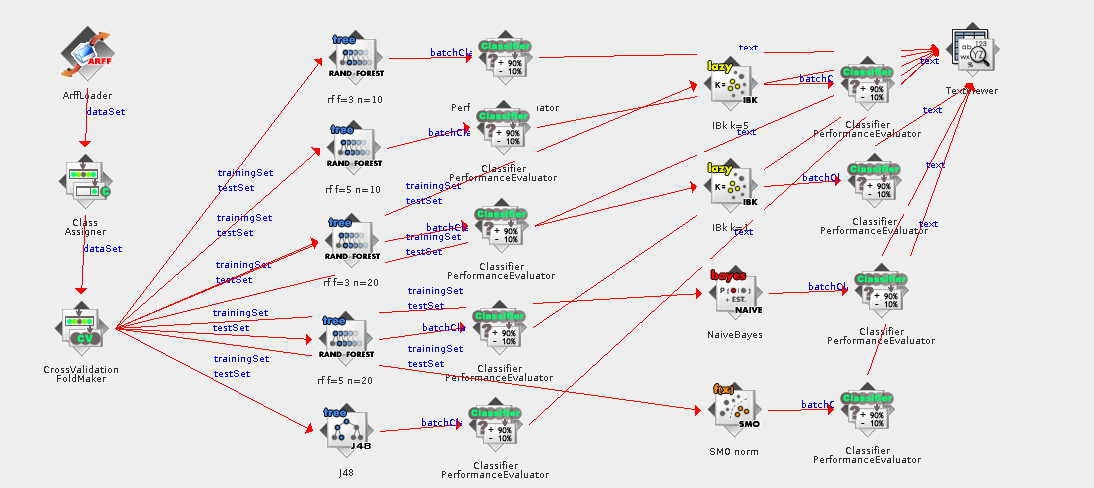
\includegraphics[angle=90, scale=0.9]{liver_kf}
\caption{\label{fig:knfilpd}Knowledge flow for the ILPD data set}
\end{figure}

We have trained four different random forrest classifiers and used two different
kNN classifiers. As visible in the image, we used no special coding for the one
categorical attribute (gender). All of the used classifiers support categorical
data. For the random foresst classifier we trained two foressts with ten trees
and two forrests. Of those two foressts one used three attributes and one five. 
We also used a kNN classifier with $k=1$ and $k=5$. We also tried higher values
for $k$, without better results. Since those nodes cluttered the flow even more
we deleted those. 

\begin{table}
\begin{tabular}{|l| c | c | c | c |}
\hline & & & & \\
Algorithms & Param. & Cor. Classified & Mean absolute & Root mean \\
& & & error & square error\\
\hline & & & & \\
   J48 &-C 0.25 -M 2 (default) & 68.78\% & 0.3292 & 0.4814 \\
\hline & & & & \\
NaiveBayes & (default) & 55.75\% & 0.4407 & 0.6541 \\
\hline & & & & \\
       SMO & (default) & 71.36\% & 0.2864 & 0.5352 \\
\hline & & & & \\
    RandomForest & -I 10 -K 3 -S 1 & 73.07\% & 0.3276 & 0.4300 \\
\hline & & & & \\
    RandomForest & -I 10 -K 5 -S 1 & 68.61\% & 0.3451 & 0.4491 \\
\hline & & & & \\
    RandomForest & -I 20 -K 3 -S 1 & 72.21\% & 0.3304 & 0.4222 \\
\hline & & & & \\
    RandomForest & -I 20 -K 5 -S 1 & 69.98\% & 0.3404 & 0.4355 \\
\hline & & & & \\
    IBk          & -K 1 (rest default) & 64.15\% & 0.3590 & 0.5976 \\
\hline & & & & \\
    IBk          & -K 5 (rest default) & 64.32\% & 0.3802 & 0.4699 \\
\hline 
\end{tabular}
\end{table}
We couldn't figure out how to measure the training time in knowledge flow, but
this dataset was very small anyway and the calculation of the whole flow came to a halt after very
few seconds. Interestingly the best result regarding corectly classified
instances was the smallest (regarding number of attributs and number of trees)
random forest classifier. We belive that the bigger forests had not enough
variance. 

\subsection{Echocardiogram data set}
The Echocardiogram data set is the smallest dataset, which has around 132
instances. We decided to use the knowledge flow feature for this dataset to.
As a first step we converted the \emph{csv} file to a \emph{arff} file as
before. For reference we give the header here.
\begin{verbatim}
@relation echocardiogram

@attribute survival numeric
@attribute still-alive {1,0}
@attribute age-at-heart-attack numeric
@attribute pericardial-effusion {1,0}
@attribute fractional-shortening numeric
@attribute epss numeric
@attribute lvdd numeric
@attribute wall-motion-score numeric
@attribute wall-motion-index numeric
@attribute mult numeric
@attribute name {name}
@attribute group numeric
@attribute alive-at-1 {1,0}
\end{verbatim}

This data contains many missing values in most attributes.
The most of the missing values are in the last column, which can
also be the class attribute. 58 of the values are missing and it is almost
half of the instances. The first attribute (survival) is a bit missleading
we susbect that it tells us how long after the
attack the record of the patient was recorded. Some of the patients are still
alive, therefore this column doesn't tell us how long the patient survived. 
The last columes is a result of the first two, and
indicates if the patient was/is still alive one year after a attack. 

For all those  reasons, we have chosen the still alive column as
the class attribute instead of alive-at-1. This is suggested by the description
of the data set. Since the alive-at-1 attreibute is a result of the first two,
we removed this attribute. Futhermore the description of the data set suggests
to remove the wall-motion-score and the group attribute. Since the name
attribute is allways \emph{name}, because the data set is anonymised, we removed
this column to. A \emph{Remove} node can be used in the knowledge flow to do
this task. 

Since there are missing values in most of the attributes left, we used a
\emph{ReplaceMissingValues} node. It replaces missing values with the mean for
numerical attributes and the mode (the value which occurs most often) for nominal
attributes. Since all the algorithms could handel missing values by themselfes
we run the classification task without the preprocessing node.
The first table shows the results with the preprocessing step, the second one
without.
\begin{table}
\begin{tabular}{|l| c | c | c | c |}
\hline & & & & \\
Algorithms & Param. & Cor. Classified & Mean absolute & Root mean \\
& & & error & square error\\
\hline & & & & \\
J48 &-C 0.25 -M 2 (default) & 88.55\% & 0.1601 & 0.3308 \\
\hline & & & & \\
NaiveBayes & (default) & 84.73\% & 0.1699 & 0.3406 \\
\hline & & & & \\
   SMO & (default) & 87.02\% & 0.1298 & 0.3602 \\
\hline & & & & \\
RandomForest & -I 10 -K 3 -S 1 & 88.55\% & 0.1618 & 0.2812 \\
\hline & & & & \\
RandomForest & -I 10 -K 5 -S 1 & 87.02\% & 0.1458 & 0.2967 \\
\hline & & & & \\
RandomForest & -I 20 -K 3 -S 1 & 89.31\% & 0.1637 & 0.2800 \\
\hline & & & & \\
RandomForest & -I 20 -K 5 -S 1 & 88.55\% & 0.1504 & 0.2886 \\
\hline & & & & \\
IBk          & -K 1 (rest default) & 80.92\% & 0.1960 & 0.4333 \\
\hline & & & & \\
IBk          & -K 5 (rest default) & 84.73\% & 0.2406 & 0.3559 \\
\hline 
\end{tabular}
\end{table}

\begin{table}
\begin{tabular}{|l| c | c | c | c |}
\hline & & & & \\
Algorithms & Param. & Cor. Classified & Mean absolute & Root mean \\
& & & error & square error\\
\hline & & & & \\
J48 &-C 0.25 -M 2 (default) & 90.08\% & 0.1493 & 0.2979 \\
\hline & & & & \\
NaiveBayes & (default) & 85.49\% & 0.1684 & 0.3411 \\
\hline & & & & \\
   SMO & (default) & 87.02\% & 0.1298 & 0.3602 \\
\hline & & & & \\
RandomForest & -I 10 -K 3 -S 1 & 89.31\% & 0.1503 & 0.2841 \\
\hline & & & & \\
RandomForest & -I 10 -K 5 -S 1 & 89.31\% & 0.1501 & 0.3022 \\
\hline & & & & \\
RandomForest & -I 20 -K 3 -S 1 & 89.31\% & 0.1556 & 0.2837 \\
\hline & & & & \\
RandomForest & -I 20 -K 5 -S 1 & 90.84\% & 0.1467 & 0.2831 \\
\hline & & & & \\
IBk          & -K 1 (rest default) & 77.10\% & 0.2335 & 0.4746 \\
\hline & & & & \\
IBk          & -K 5 (rest default) & 81.68\% & 0.2375 & 0.3567 \\
\hline 
\end{tabular}
\end{table}

For the J48 and NaiveBayes algorithms the build in handling gives better
results. For the support vector maschine algorithm we get exactly the same
results and only the two variants of kNN classifiers give worse results.
\subsection{Comparison}

\section{Conclusion}

\end{document}
